\scanpage{58}

\[u_r:\widetilde G_3\xrightarrow{\sim}\widetilde G_3\]

et tout repère $r'$ \inserted{\unsure{avec $=$ $\varepsilon$ que $r$|au $=$ $\varepsilon$ près|avec $=$ $\varepsilon$ pour $r$}} sera de la forme de façon unique

\[r'=rg_0\quad\text{avec }g_0\in\widetilde G_3\]

\[(38)\quad\text{ie.}\quad u_{r'}=u_ru_{g_0}\qquad(\text{avec }u_r(g_0)=g\text{ mais peu importe})\]

d'où, en passant à l'action sur les $\Pi_1$ en $P_+$ resp. $P_\varepsilon$, on trouve

\[(39)\qquad\psi_{r'\deleted{\unsure{\varepsilon}}}=\psi_r\circ\Pi_1(g_0,P_+)\qquad\text{si }r'=r\circ g_0\]

\margin{$\psi_r,\psi_{r'}$ désignent ici les isom\unsure{s}\unsure{.} d'épin-\linebreak glage associés \deleted{aux} à $P_\varepsilon$}

On va expliciter ceci pour

\[g_0=\rho\quad\text{donc }r'=r\rho=(\omega i,\omega,\bar\omega)\quad\text{si }r=(i,\omega,\bar\omega)\]

On trouve

\[\psi_\varepsilon^{\omega i,\omega}=\overset{\inserted{\rho_\omega\circ\psi_\varepsilon^{i,\omega}=}}{\psi_\varepsilon^{i,\omega}\circ\rho}\]

où on a identifié $\rho$ aussi à un élément de $\widetilde\Pi_{0,3}$, et à l'autom qu'il induit sur $\Pi_{0,3}$

\uline{NB} $\rho_\omega$ est la rotation autour de $P_\varepsilon,P_{\varepsilon'}$ d'un tiers de tour, \deleted{\unsure{suivant}} l'orientation $\omega$ sur l'équateur

\margin{\uline{NB}\quad $\psi_\varepsilon^{\unsure{i|\omega},\omega}(l_0),\psi_\varepsilon^{i,\omega}(l_1),\deleted{\unsure{\psi_\varepsilon^{i,\omega}(l_0)}}$ \unsure{sont} resp. les lacets \unsure{fondés|standard|tournant} à partir de $P_\varepsilon$, autour des trous $R_{\omega i},R_{\omega^2 i}$, \deleted{\unsure{qui}} passant $Q_i$ (donc \unsure{au détriment de} $\unsure{R_{\omega i}|R_{\omega\prime i}}$ : $\unsure{R_{\omega\prime i}\cdots|R_{\omega^2 i}\cdots|R_{\omega i}\cdots}$), et dans le sens d'orientation $\bar\omega=\omega\wedge\varepsilon$}

\figure{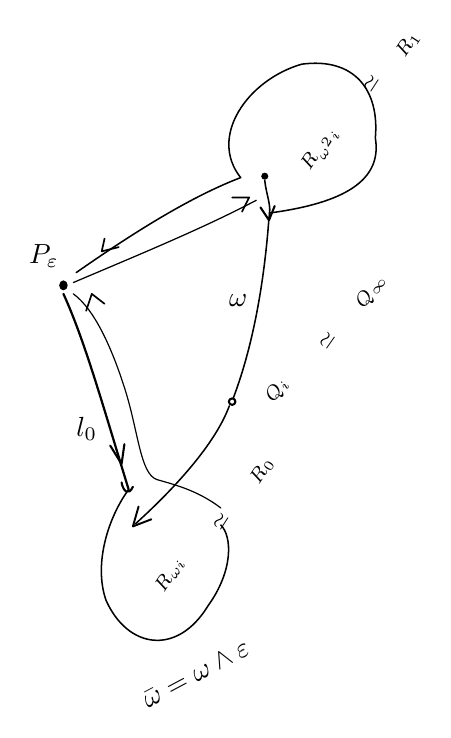
\begin{tikzpicture}[x=.018cm,y=-.018cm,line cap=round,line join=round]
\draw[line width=.55pt] (204,1700) .. controls (181,1671) and (209,1631) .. (247,1620) .. controls (284,1615) and (302,1638) .. (299,1672) .. controls (304,1702) and (277,1718) .. (224,1725);
\draw[line width=.55pt] (125,1920) .. controls (111,1939) and (100,1972) .. (109,1998) .. controls (124,2032) and (159,2038) .. (181,2002) .. controls (199,1977) and (198,1953) .. (190,1945);
\draw[line width=.55pt] (204,1700) .. controls (170,1713) and (131,1737) .. (88,1767);
\draw[line width=.60pt] (108,1743) -- (106,1752) -- (118,1749);
\draw[line width=.45pt] (86,1774) .. controls (133,1754) and (177,1736) .. (215,1716);
\draw[line width=.60pt] (198,1714) -- (210,1714) -- (205,1724);
\draw[line width=.80pt] (79,1782) .. controls (94,1815) and (106,1858) .. (125,1920);
\draw[line width=.75pt] (112,1889) -- (120,1902) -- (122,1888);
\draw[line width=.75pt] (120,1915) .. controls (121,1921) and (125,1925) .. (128,1918);
\draw[line width=.43pt] (190,1933) .. controls (173,1920) and (155,1916) .. (145,1913) .. controls (133,1909) and (132,1879) .. (122,1848) .. controls (113,1820) and (101,1793) .. (86,1782);
\draw[line width=.60pt] (95,1794) -- (99,1782) -- (108,1789);
\draw[line width=.56pt] (221,1702) .. controls (222,1712) and (226,1720) .. (224,1728) .. controls (221,1769) and (214,1815) .. (199,1855);
\draw[line width=.75pt] (218,1721) -- (224,1730) -- (228,1720);
\draw[line width=.55pt] (196,1861) .. controls (185,1891) and (151,1925) .. (130,1944);
\draw[line width=.70pt] (132,1932) -- (128,1946) -- (141,1941);
\fill (79,1776) ellipse[x radius=3.0,y radius=3.5];
\fill (221,1699) circle[radius=2.5];
\draw[line width=.75pt,fill=white] (198,1858) circle[radius=2.3];
\node[anchor=south east,inner sep=.5pt] at (77,1765) {$P_\varepsilon$};
\node[anchor=center,rotate=55,font=\scriptsize,inner sep=.2pt] at (230,1850) {$Q_i$};
\node[anchor=center,rotate=55,font=\scriptsize,inner sep=.2pt] at (265,1815) {$\simeq$};
\node[anchor=center,rotate=55,font=\scriptsize,inner sep=.2pt] at (296,1780) {$Q_\infty$};
\node[anchor=center,rotate=57,font=\scriptsize,inner sep=.2pt] at (260,1680) {$R_{\omega^2 i}$};
\node[anchor=center,rotate=57,font=\scriptsize,inner sep=.2pt] at (296,1634) {$\simeq$};
\node[anchor=center,rotate=57,font=\scriptsize,inner sep=.2pt] at (322,1606) {$R_1$};
\node[anchor=center,rotate=57,font=\scriptsize,inner sep=.2pt] at (154,1980) {$R_{\omega i}$};
\node[anchor=center,rotate=57,font=\scriptsize,inner sep=.2pt] at (190,1943) {$\simeq$};
\node[anchor=center,rotate=57,font=\scriptsize,inner sep=.2pt] at (219,1907) {$R_0$};
\node[anchor=east,inner sep=.5pt] at (104,1877) {$l_0$};
\node[anchor=east,inner sep=.5pt] at (210,1787) {$\omega$};
\node[anchor=west,rotate=28,inner sep=.5pt] at (135,2070) {$\bar\omega=\omega\wedge\varepsilon$};
\end{tikzpicture}}

On trouve de $=$, pour un autom qui renverse l'orientation de $\sigma$ i.e. pour un

\[\widetilde\sigma_\infty:\quad\begin{array}{rcl}0&\longrightarrow&1\\1&\longrightarrow&0\\{}^{\unsure{\prime}}\!\infty&\longrightarrow&\infty\end{array}\qquad\deleted{\unsure{\text{la}}}\deleted{\unsure{\text{pour}|\longmapsto}}\bar\omega\longmapsto\bar\omega'\]

\deleted{$\unsure{\widetilde\sigma_\infty}$}

\[g_0=\widetilde\sigma_\infty\qquad r'=r\sigma_\infty=(\deleted{\unsure{\omega}}i,\omega',\bar\omega').\]

d'où

\[(41)\qquad\psi_\varepsilon^{\deleted{\unsure{\omega}}i,\omega'}=\overset{\inserted{\widetilde\sigma_{\unsure{\deleted{\infty}i|i}}\circ\psi_\varepsilon^{i,\omega}=}}{\psi_\varepsilon^{i,\omega}\circ\widetilde\sigma_\infty}\]

($\widetilde\sigma_i$ est la symétrie p.r. \unsure{au|du} grand cercle méridien passant par $Q_i$)

\margin{57}
